\Chapter{Tervezés}
\Section{Modellek}

Modellek kapcsán első lépésben összegyűjtöttem számos OBJ file-t, egy részüknek az adatait \aref{fig:modellekt} táblázatban összegyűjtöttem.

\begin{table}[h]
\centering
\caption{Modellek táblázat}
\bigskip
\label{tab:modellek}
\begin{tabular}{|l|c|c|c|c|c|c|c|c|}
Modell neve& Vektor & T.vektor & N.vektor & Arc & H.szög & N.szög \\
\hline
baby.obj & 12030 & 13154 & 12030 & 12028 & 0 & 12028 \\
barrel.obj & 9348 & 9674 & 5411 & 5887 & 0 & 5880	\\
bird.obj & 8758 & 9582 & 8685 & 8752 & 0 & 8752 \\
boat.obj & 102669 & 203174 & 66538 & 100624 & 1294 & 99330\\
butterfly.obj & 1394 &	8328 &	0 & 2776 &	2776 &	0 \\
camera.obj & 17000 & 18580 & 16788 & 16984 & 0 & 16984 \\
cat.obj & 35290 & 36525 & 35014 & 35288 & 0 &	35288 \\
chair.obj & 78906 & 111336 & 45764 & 83074 & 11352 & 71722 \\
coral.obj & 43212 & 51349 & 43211 & 43200 & 0 & 43200 \\
cube.obj & 8 & 4 & 6 & 12 & 12 & 0 \\
deer.obj & 39402 & 41696 & 38642 & 39384 & 0 & 39384 \\
dog.obj & 35986 & 37096 & 35983 & 35984 & 0 & 35984 \\
dolphin.obj & 7338 & 7815 & 7337 & 7336 & 0 & 7336 \\
door.obj & 2058 & 2456 & 629 & 2152 &	220 & 1932 \\
lion.obj & 64558 & 67131 & 64556 & 64536 & 0 & 64536 \\
monkey.obj & 47490 & 49505 & 47490 & 47488 & 0 & 47488 \\
necklace.obj & 85592 &	94527 & 83931 & 85592 & 0 & 85592 \\
penguin.obj & 7494 & 7961 & 7493 & 7488 & 0 & 7488 \\
skull.obj & 40062 & 42682 & 40062 & 40728 & 1440 & 39288 \\
wrench.obj & 11568 & 13326 & 10508 & 11568 & 0 & 11568 \\
\hline
\end{tabular}
\label{fig:modellekt}
\end{table}

\Aref{fig:modellekt} tábázat modelleit a \url{https://free3d.com/} oldalról gyűjtöttem be. Ahol rengetek modell megtalálható. Ezeken a modelleken fellépő hibákat illetve különböző modellek kompatibilitási problémát vizsgáltam.\\

Vizsgálat során az  első szembetűnő dolog az volt, hogy ezek az objektumok komplexitásukban, jelentősen eltérnek egymástól. Voltak köztük olyan objektumok, amik viszonylag kevés komponensből állnak össze és voltak olyanok is, amik ezekhez képest jelentősen több elemből.
Természetesen az oldalon található modell fájlok többsége teljesen jól működik, de akadtak köztük hibásak is.\\

Majd rendszereztem őket az alábbi kategóriákba:
\begin{itemize}
\item Helyes modellek:\\
A megjelenítés tökéletesen megtörtént.
\bigskip
\item Javítható hibák:\\
A modellnek olyan javítható hibája van, ami a program segítségével majd javításra kerülhet.
\bigskip
\item Nem javítható hibák:\\
A modellnek olyan hibája van, ami nem kerülhet javításra a program segítségével.
\end{itemize}
\bigskip

\newpage

\Section{Saját Modell Struktúra Megtervezése}

\noindent Ennél a lépésnél megvizsgáltam és figyelembe vettem az általam vizsgált modell betöltők struktúrális felépítését és a következő konzekvenciát szűrtem le:\\

Az általam megvizsgált modellbetöltők tárolási módjai elég hasonlóak. Az objektum adataid egy közös modell struktúrában tárolják, ezt feltöltő adatokat pedig al struktúrákban.\\

A .obj model adatait egy közös model struktúrában tárolja a program a struktúrák egymás közötti felépítése \aref{fig:struct}-es ábrán látható.
\bigskip
\begin{figure}[h]
\centering
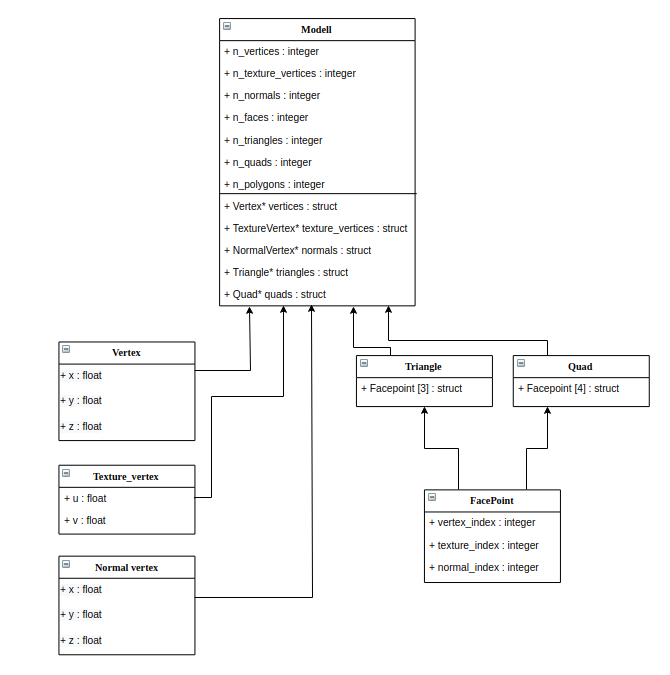
\includegraphics[width=\textwidth]{images/struct.png}
\caption{Model Struktúra.}
\label{fig:struct}
\end{figure}
\bigskip

Az integer típusú \texttt{n\_vertices}, \texttt{n\_texture\_vertices}, \texttt{n\_normals}, \texttt{n\_faces} illetve \texttt{n\_triangles}, \texttt{n\_quads} és \texttt{n\_polygons} változók feltöltésre kerülnek az OBJ fájl különböző változótípus darabasznámainak összeszámlálásával.
\begin{python}
typedef struct Model
{
    int n_vertices;
    int n_texture_vertices;
    int n_normals;
    int n_faces;
    int n_triangles;
    int n_quads;
    int n_polygons;
}Model
\end{python}
\bigskip

Ezt követően a \texttt{n\_vertices} számával közvetlen kiolvasásra kerülnek a \texttt{Vertex} struktúra különböző csúcspontjai.
\begin{python} 
typedef struct Vertex
{
    double x;
    double y;
    double z;
}Vertex;
\end{python}
\bigskip

Hasonlóan a Vertex struktúrához a \texttt{TextureVertex} csúcspontjai is kiolvasásra kerülnek az \texttt{n\_texture\_vertices} darabszámaival.
\begin{python}
typedef struct TextureVertex
{
    double u;
    double v;
}TextureVertex;
\end{python}
\bigskip

Majd az előzőekhez hasonlóan a \texttt{NormalVertex}  struktúra csúcspontjai is feltöltődnek az \texttt{n\_normals} darabszámmal.
\begin{python}
typedef struct NormalVertex
{
    double x;
    double y;
    double z;
}NormalVertex;
\end{python}
\bigskip
\newpage
Végül a \texttt{Triangle} és \texttt{Quad} struktúrák is feltöltésre kerülnek, \texttt{FacePoint} struktúra segítségével.
\begin{python}
typedef struct FacePoint
{
    int vertex_index;
    int texture_index;
    int normal_index;
} FacePoint;

typedef struct Triangle
{
    struct FacePoint points[3];
} Triangle;

typedef struct Quad
{
    struct FacePoint points[4];
} Quad;
\end{python}
\bigskip

Az összes adat  \texttt{Model} struktúrában kerül eltárolásra ennek előnye, hogy egy közös, kap helyet az OBJ fájl összes fontos adata, így egyszerűbben lehet rájuk hivatkozni illetve a modellen történő szükséges változásokat  így könnyebben elvégezhetjük
\begin{python}
typedef struct Model
{
    int n_vertices;
    int n_texture_vertices;
    int n_normals;
    int n_faces;
    int n_triangles;
    int n_quads;
    int n_polygons;
    struct Vertex* vertices;
    struct TextureVertex* texture_vertices;
    struct NormalVertex* normals;
    struct Triangle* triangles;
    struct Quad* quads;
}Model;
\end{python}
\newpage
\Section{Elem indexelés}

\bigskip
\begin{figure}[h]
\centering
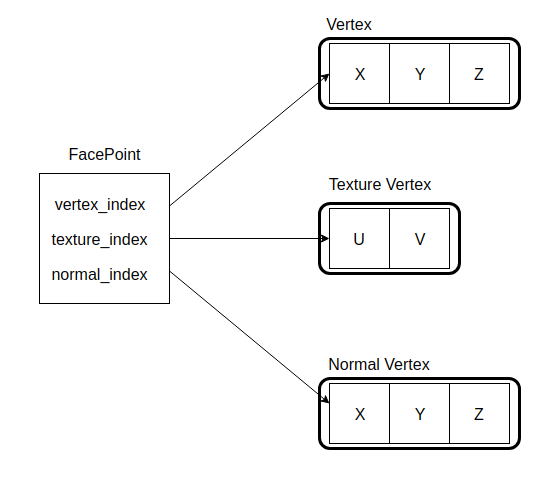
\includegraphics[scale=0.5]{images/point.png}
\caption{Model Struktúra.}
\label{fig:index_}
\end{figure}
\bigskip

\Aref{fig:index_} ábrán megtervezésre került egyes arcelemek hogyan fognak mutatni a különböző vektorok koordinátájra. Ennek a segítségével fogja a program összeállítani a síkodomokat.


%\Section{Betöltők tárolási módjai}
%\Section{Modellek}
%\Section{Saját modell struktúra}
